\documentclass{oci}
\usepackage[utf8]{inputenc}
\usepackage{lipsum}

\title{Transbordo en el aeropuerto}

\begin{document}
\begin{problemDescription}
  A Lucas le encanta viajar.
  Lo hace varias veces al año, escogiendo siempre un nuevo destino. % para conocer.
  Para ahorrar dinero y así poder viajar más, Lucas siempre toma los vuelos más
  baratos.
  Esto suele ser un problema pues a menudo tiene que realizar escalas y correr
  para alcanzar el siguiente avión.

  Los aeropuertos siempre están divididos en \emph{terminales}.
  Cuando Lucas se baja de un avión lo hace en un terminal de \emph{llegada} y
  tiene que recorrer el aeropuerto rápidamente hasta llegar al terminal de \emph{salida} de su próximo vuelo.
  Los terminales dentro de un aeropuerto están conectados por conexiones que Lucas
  puede atravesar caminando en ambos sentidos.
  Para hacer más rápido el recorrido algunos aeropuertos cuentan con 
  trenes entre algunos terminales.
  
  Después de tantos viajes Lucas conoce prácticamente todos los aeropuertos
  y tiene mapas de cada uno, con las conexiones entre terminales
  junto con el tiempo que tarda en recorrerlas caminando, 
  más toda la información de trenes entre terminales.
  Más aun, cuenta con información del momento en que los trenes partirán de cada
  terminal y el tiempo que tardan en llegar al terminal donde se dirigen.
  
%  Muchas veces es imposible recorrer los aeropuertos solo caminando así que
%  estos ponen a disposición trenes entre algunos terminales.
%  Lucas también tiene la información de estos trenes y sabe 
%  el momento exacto en que los trenes partirán de cada
%  terminal y el tiempo que tardarán en llegar al terminal donde se dirigen.

  La siguiente figura muestra un mapa de un aeropuerto %de ejemplo 
  con tres terminales.
  
  \begin{center}
  \includegraphics[scale=0.7]{aeropuerto}
  \end{center}  
  
  Las líneas continuas representan las conexiones que Lucas puede atravesar
  caminando, y el número junto a la conexión representa el tiempo en minutos que Lucas tarda
  en caminar de un extremo al otro. Por ejemplo, Lucas puede ir caminando del terminal $2$ al $1$
  y tardará $5$ minutos. También puede caminar del $2$ al $3$ tardando 20 minutos.
  Las líneas punteadas indican los trayectos en tren.
  Estos trayectos están descritos por dos números. El primero de ellos
  representa el momento en que el tren comenzará su recorrido 
  medido como la cantidad de minutos desde que Lucas llega al aeropuerto.
  El segundo corresponde al tiempo en minutos que el tren tardará en
  completar el recorrido.
  Por ejemplo, considere el tren que se mueve del terminal $1$ al $3$, y que está
  descrito por los valores $(30, 5)$. El $30$ indica que el tren comenzará su recorrido 
  $30$ minutos después de que Lucas llega al aeropuerto, y el $5$ indica que el tren tardará $5$ minutos
  en recorrer del terminal $1$ al $3$.
  Similarmente, la figura muestra que hay dos trenes que se mueven del terminal $2$ al terminal $3$, descritos por los pares $(3,6)$ y $(6,7)$.
  El primero de ellos comienza su recorrido $3$ minutos después de que Lucas llega al aeropuerto y tarda $6$ minutos en completarlo.
  El segundo comienza $6$ minutos después de que Lucas llega al aeropuerto y tarda $7$ en completar el recorrido.
  Finalmente, note que el tren que viaja del terminal 
  $3$ al terminal $1$ comienza su recorrido justo en el momento
  que Lucas llega al aeropuerto, pues está descrito por $(0,5)$.

  Suponga que el avión de Lucas llega al terminal $1$ y su próximo vuelo sale desde
  el terminal $3$. ¿Cuál es el menor tiempo en que Lucas puede llegar desde uno al otro?
  Notemos que tiene varias
  alternativas.
  La primera es esperar 30 minutos a que el tren parta desde el terminal 1 hacia
  el 3.
  Estos 30 minutos de espera más los 5 minutos que tarda el tren dan un total de
  35 minutos para el recorrido.
  Otra alternativa es caminar hacia el terminal 2 tardando 5 minutos.
  En este momento Lucas ya perdió la posibilidad de tomar el primer tren que
  parte de está estación, pero puede esperar un minuto y tomar el segundo tren.
  Contando los 7 minutos que este tarda en llegar a su destino da un total de 13
  minutos para moverse desde el terminal $1$ al $3$.
  La última alternativa es caminar primero del terminal $1$ al $2$ ($5$ minutos) 
  y luego seguir caminando desde el $2$ al $3$ ($20$ minutos) 
  tardando un total de 25 minutos.
  Por lo tanto, en el mejor caso Lucas tarda $13$ minutos en llegar al terminal $3$.

  Lucas ya está cansado de perder vuelos y necesita tu ayuda.
  Dada la descripción de un aeropuerto, el terminal $A$ de llegada del vuelo de Lucas y el terminal $B$
  de salida de su próximo vuelo, tu tarea es calcular el menor tiempo en que es posible
  trasladarse desde $A$ a $B$.
  

\end{problemDescription}

\begin{inputDescription}
  La primera línea de la entrada contiene cuatro enteros $N$, $M$, $A$ y $B$
  ($0 < N\leq 1000, 0 < M \leq 10000$, $1 \leq A, B\leq N$).
  Los enteros $N$ y $M$ corresponden respectivamente a la cantidad de terminales
  y de conexiones para caminar entre los terminales.
  Cada terminal es identificado con un número entre 1 y $N$.
  Los enteros $A$ y $B$ corresponden respectivamente al terminal de llegada del vuelo de Lucas 
  y al terminal de salida de su siguiente vuelo.

  Posteriormente, cada una de las siguientes $M$ líneas contienen tres enteros
  $u$, $v$ y $c$ ($1\leq u, v\leq N$ y $0<c\leq 1000$), indicando que existe una
  conexión entre el terminal $u$ y el terminal $v$ y que Lucas tarda $c$ minutos
  en recorrerla caminando.
  Se garantiza que siempre será posible moverse entre cualquier par de
  terminales usando solamente estas conexiones.

  A continuación sigue una línea con un entero $P$ correspondiente a la
  cantidad de entradas que contiene el itinerario de viajes en tren.
  Cada una de las siguientes $P$ líneas contiene cuatro enteros $u$, $v$,
  $t$ y $w$ ($1 \leq u,v \leq N, 0\leq t\leq 10^9, 0 < w \leq 1000$)
  describiendo un trayecto en tren. 
  Los enteros indican que el tren viajará desde el terminal $u$ hasta el
  terminal $v$, que partirá $t$ minutos después de que Lucas llega al aeropuerto
  y que este se demora $w$ minutos en viajar de $u$ a $v$.
\end{inputDescription}

\begin{outputDescription}
  La salida debe contener un solo entero correspondiente al tiempo mínimo en que
  Lucas puede llegar desde $A$ a $B$.
\end{outputDescription}

\begin{scoreDescription}
  \score{5} Se probarán varios casos en que no hay trayectos en tren ($P=0$) y
  las conexiones entre terminales formarán una línea, es decir, el primer
  terminal está conectado al segundo, el segundo con el tercero, etc (ver
  el primer ejemplo de entrada). 
  \score{10} Se probarán varios casos en que las conexiones entre terminales formarán una línea 
  como en la subtarea anterior, pero además es posible que hayan
  trayectos en tren entre terminales consecutivos, es decir, puede haber un
  tren entre el terminal $i$ y el $i+1$ o entre el $i+1$ y el $i$ (ver segundo
  ejemplo de entrada).
  \score{35} Se probarán varios casos sin trayectos en tren ($P=0$) y sin
  restricciones en las conexiones (ver tercer ejemplo de entrada).
  \score{50} Se probarán varios casos sin restricciones adicionales (ver cuarto
  ejemplo de entrada).
\end{scoreDescription}

\begin{sampleDescription}
\sampleIO{sample-1}
\sampleIO{sample-2}
\sampleIO{sample-3}
\sampleIO{sample-4}
\end{sampleDescription}

\end{document}
